\documentclass[UTF8]{ctexart}
%%%%%%%%%%%%%%%%%%%%%%%%%%%== 引入宏 ==%%%%%%%%%%%%%%%%%%%%%%%%%%%%%
\usepackage{cite}
\usepackage{amsmath}	% 使用数学公式
\usepackage{graphicx}	% 插入图片/PDF/EPS 等图像
\usepackage{geometry}	% 设置页边距
\usepackage{fancyhdr}	% 设置页眉页脚
\usepackage{setspace}	% 设置行间距
\usepackage{hyperref}	% 让生成的文章目录有链接,点击时会自动跳转到该章节
\usepackage{url}
\usepackage{caption2}
\usepackage{ulem}
\usepackage{listings}
\usepackage{xcolor}
\usepackage[T1]{fontenc}
\usepackage{textcomp}
\usepackage[utf8]{inputenc}
\lstset{
 columns=fixed,
 numbers=left,                                        % 在左侧显示行号
 numberstyle=\tiny\color{gray},                       % 设定行号格式
 frame=none,                                          % 不显示背景边框
 backgroundcolor=\color[RGB]{245,245,244},            % 设定背景颜色
 keywordstyle=\color[RGB]{40,40,255},                 % 设定关键字颜色
 numberstyle=\footnotesize\color{darkgray},
 commentstyle=\it\color[RGB]{0,96,96},                % 设置代码注释的格式
 stringstyle=\rmfamily\slshape\color[RGB]{128,0,0},   % 设置字符串格式
 showstringspaces=false,                              % 不显示字符串中的空格
 language=Python,                                        % 设置语言
}


%%%%%%%%%%%%%%%%%%%%%%%%%%== 设置全局环境 ==%%%%%%%%%%%%%%%%%%%%%%%%%%%%
% [geometry] 设置页边距
\geometry{top=2.6cm, bottom=2.6cm, left=2.45cm, right=2.45cm, headsep=0.4cm, foot=1.12cm}
% 设置行间距为 1.5 倍行距
\onehalfspacing
% 设置页眉页脚
\pagestyle{fancy}
%\lhead{左头标}
%\chead{\today}
%\rhead{152xxxxxxxx}
\lfoot{}
\cfoot{\thepage}
\rfoot{}
%\renewcommand{\headrulewidth}{0.4pt}
%\renewcommand{\headwidth}{\textwidth}
%\renewcommand{\footrulewidth}{0pt}

%%%%%%%%%%%%%%%%%%%%%%%%%%== 自定义命令  ==%%%%%%%%%%%%%%%%%%%%%%%%%%%%%%
% 此行使文献引用以上标形式显示
\newcommand{\supercite}[1]{\textsuperscript{\cite{#1}}}
% 此行使section中的图、表、公式编号以A-B的形式显示

% 此行使图注、表注与编号之间的分隔符缺省,默认是冒号:
\renewcommand{\captionlabeldelim}{~}

%===================================== 标题设置  ==========================================
% \heiti \kaishu 为字体设置,ctex 会自动根据操作系统加载字体
\author{\small{\kaishu 71118415 叶宏庭}\\[2pt]
\small{\kaishu 东南大学软件学院}\\[2pt]
\small{Email:}
\url{213182964@seu.edu.cn}
}
\title{\Huge{\heiti 多播聊天工具}}
\CTEXoptions[today=old]
\date{\today} % 去除默认日期
%\date{\today}

%===================================== 正文区域  ==========================================
\begin{document}
\maketitle

\section{实验目的}{通过课程学习,已经对多播原理有了初步的了解,接下来要做的便是完成具体的编程实现,本次大作业选择完成一个带有文件传输功能的多播聊天工具,具体要求如下: }
\par{
	\begin{itemize}
		\item[*] 支持字符的传输,也就是聊天文本的传输。
		\item[*] 支持文件的传输,例如:源通过多播方式将文件发送给多个接收方,接收方收到后,能够正常打开。
		\item[*] 能够对多播组成员进行管理(如何实现当前多播组成员的显示、删除等功能?)。
	\end{itemize}
}

\section{实验环境}
\subsection{操作系统:}{Windows 10, Windows 7}
\subsection{编译环境:}{Python 3.7, Pyinstaller 4.3}
\subsection{辅助软件:}{TexLive(用于编写tex报告),VS code(用于编写程序)}
\section{实验内容}
\subsection{聊天界面设计:}{设计一个简单实用,简洁明了的UI界面,形成一个完整的聊天工具。}
\par\centerline{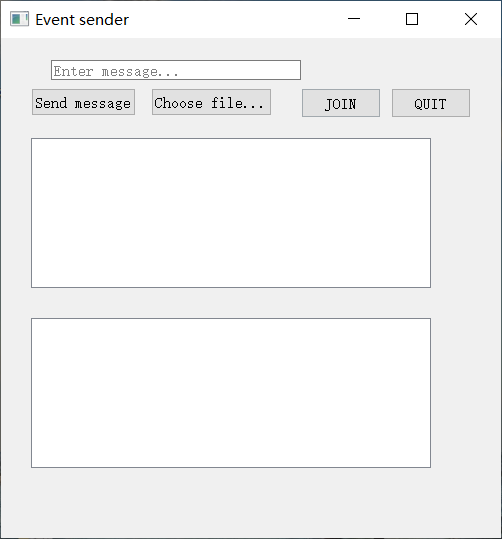
\includegraphics[scale=0.6]{UI.png}}
\par{如上图所示,界面中包含了一个输入框,用于输入文本信息,提供了四个按钮,分别是消息发送按钮,文件选择按钮,JOIN加入组播按钮,QUIT退出组播按钮。在下方有两个列表视图,第一个为消息列表视图,用于显示消息,第二个为多播组成员列表视图,用于显示多播组成员信息。
}
\subsection{核心代码实现:}{本部分将介绍该程序的核心代码,包括网络配置、消息发送与接收、文件发送与接收、多播组成员管理、JOIN与QUIT操作。}
\subsubsection{网络配置:}{首先,给出网络配置的核心代码:}
\par{
\begin{lstlisting}
# 定义组播网络参数
ANY = '0.0.0.0'
SENDERPORT=1501                     # 发送消息所用端口
MCAST_ADDR = '224.168.2.9'          # 组播消息地址
MCAST_ADDR_FILE = '235.2.3.4'       # 组播文件地址
MCAST_PORT_MSG = 1600               # 组播消息端口
MCAST_PORT_FILE = 1700              # 组播文件端口

# 初始化网络参数
def initNetConfig(self):
	# 修改链接标志位
	self.connect_flag = True
	
	# 配置发送套接字
	self.send_sock = socket.socket(
			socket.AF_INET, socket.SOCK_DGRAM, socket.IPPROTO_UDP) 
	#允许端口复用 
	self.send_sock.setsockopt(
			socket.SOL_SOCKET,socket.SO_REUSEADDR,1)
	#绑定发送端口到SENDERPORT,即此例的发送端口为1501
	self.send_sock.bind(
			(ANY,SENDERPORT)) 
	#设置使用多播发送
	self.send_sock.setsockopt(
			socket.IPPROTO_IP, socket.IP_MULTICAST_TTL, 255)
	#设置回环地址
	self.send_sock.setsockopt(
			socket.IPPROTO_IP,socket.IP_MULTICAST_LOOP, False) 
	
	# 配置消息接收套接字
	self.rece_sock = socket.socket(
			socket.AF_INET, socket.SOCK_DGRAM, socket.IPPROTO_UDP) 
	#允许端口复用 
	self.rece_sock.setsockopt(
			socket.SOL_SOCKET,socket.SO_REUSEADDR,1) 
	#绑定监听多播数据包的端口
	self.rece_sock.bind((ANY,MCAST_PORT_MSG)) 
	#告诉内核这是一个多播类型的socket
	self.rece_sock.setsockopt(
			socket.IPPROTO_IP, socket.IP_MULTICAST_TTL, 255) 
	#设置回环地址
	self.rece_sock.setsockopt(
			socket.IPPROTO_IP, socket.IP_MULTICAST_LOOP, False)   
	#告诉内核把自己加入指定的多播组,组地址由第三个参数指定
	status = self.rece_sock.setsockopt(socket.IPPROTO_IP,  
			socket.IP_ADD_MEMBERSHIP, 
			socket.inet_aton(MCAST_ADDR) + socket.inet_aton(ANY));
	self.rece_sock.setblocking(0) 
	
	# 配置文件接收套接字
	self.rece_file_sock = socket.socket(
			socket.AF_INET, socket.SOCK_DGRAM, socket.IPPROTO_UDP) 
	 #允许端口复用 
	self.rece_file_sock.setsockopt(
			socket.SOL_SOCKET,socket.SO_REUSEADDR,1)
	#绑定监听多播数据包的端口
	self.rece_file_sock.bind((ANY,MCAST_PORT_FILE)) 
	#告诉内核这是一个多播类型的socket
	self.rece_file_sock.setsockopt(
			socket.IPPROTO_IP, socket.IP_MULTICAST_TTL, 255) 
	#设置回环地址
	self.rece_file_sock.setsockopt(
			socket.IPPROTO_IP, socket.IP_MULTICAST_LOOP, False) 
	 #告诉内核把自己加入指定的多播组,组地址由第三个参数指定
	status = self.rece_file_sock.setsockopt(socket.IPPROTO_IP, 
			socket.IP_ADD_MEMBERSHIP, 
			socket.inet_aton(MCAST_ADDR_FILE) + socket.inet_aton(ANY));
	self.rece_file_sock.setblocking(0) 
	
	'''
		开启监听线程
		1 user_msg:定时推送组成员信息
		2 rece_msg_thread:监听消息收取
		3 rece_file_thread:监听文件收取
	'''
	self.user_msg = _thread.start_new_thread(self.send_user_msg, ())
	self.rece_msg_thread = _thread.start_new_thread(self.rece_message, ())
	self.rece_file_thread = _thread.start_new_thread(self.rece_file, ())

\end{lstlisting}
}
\par{网络配置中,总共设计了三个socket套接字,分别用于消息或文件的发送、消息接收、文件接收。并且关闭了回环地址问题,防止形成网络风暴。在配置最后,开启了三个线程,分别用于推送成员信息(在多播组成员管理部分详细介绍)、监听消息收取、监听文件收取。
}
\subsubsection{消息发送与接收:}{首先,给出消息发送与接收的核心代码:}
\par{
\begin{lstlisting}
# 发送按钮控制函数
def sendButtonClicked(self):
    message_to_send = self.le.text()

    # TODO 发送str
    self.send_sock.sendto(
    	bytes("normal_msg#"+message_to_send, 
    	encoding="utf8"), 
    	(MCAST_ADDR,MCAST_PORT_MSG) );

    self.shows("You send: " + message_to_send)

    self.le.clear()

# 监听消息收取
def rece_message(self):
    while True: 
        if not self.connect_flag:
            break
        try: 
            data, addr = self.rece_sock.recvfrom(1024) 
            #print('hhh')
            data = bytes.decode(data).split("#")
            ctl = data[0]
            if ctl == "ctl_msg":
                # TODO 组成员更新
                if data[1] == "update":
                    if addr[0] not in self.group_mem:
                        print(addr)
                        self.group_mem.append(addr[0])
                        self.update_group_mem_list()
                elif data[1] == "QUIT":
                    if addr[0] in self.group_mem:
                        self.group_mem.remove(addr[0])
                        self.update_group_mem_list()

            else:
                self.add_items(addr, "".join(data[1:]))
        except socket.error: 
            pass 
\end{lstlisting}
}
\par{上面给出的消息发送与接收核心代码,针对不同的消息类型进行了分类,对于普通的消息信息,发送normal\_msg\#msg的格式发送,发送完成后,会在消息列表视图中加入提示信息“You sen: msg”,并且清空输入框,等待下一次输入。}
\par{对于消息收取的监听,首先利用连接标志位connect\_flag来判断是否已经退出多播组,已经退出的话,就需要break出while循环,以结束当前监听线程。在try块中,先收取data数据和addr地址信息,再根据不同的消息规定格式来进行响应的处理,包括展示消息,或者是调整多播组成员列表。
}
\subsubsection{文件发送与接收:}{首先,给出文件发送与接收的核心代码:}
\par{
	\begin{lstlisting}
# 选择文件
def choose_file(self):
    get_filename_path, ok = QFileDialog.getOpenFileName(self,
                                "选取单个文件",
                                "C:/",
                                "All Files (*);;Text Files (*.txt)")
    if ok: 
        fi = QFileInfo(get_filename_path)
        file_name = fi.fileName()
        self.get_file_result(str(file_name))
        self.sendFile(get_filename_path, file_name)
        
# 发送文件
def sendFile(self, filePath, filename):
    count = 0
    f = open(filePath, 'rb')
    while True:
        if count == 0:
            data = bytes(filename, encoding = "utf8")
            self.send_sock.sendto(data,(MCAST_ADDR_FILE,MCAST_PORT_FILE))
            print(data)
        
        data = f.read(1024)
        if str(data) != "b''":
            self.send_sock.sendto(data,(MCAST_ADDR_FILE,MCAST_PORT_FILE))
            #print(str(count)+'byte')

        else:
            self.send_sock.sendto(
            	'end'.encode('utf-8'),(MCAST_ADDR_FILE,MCAST_PORT_FILE))
            break
        #data, server_addr = self.send_sock.recvfrom(1024)
        count+=1

    self.shows(filename + " send successful!")
    
# 监听文件收取
def rece_file(self):
    while True:
        if not self.connect_flag:
            break
        filename = ''
        count = 0

        while True:
            if not self.connect_flag:
                break
            try:
                if count == 0:
                    data,client_addr = self.rece_file_sock.recvfrom(1024)
                    #print('connected from %s:%s'%client_addr)
                    filename = str(data, encoding = "utf-8")
                    print(data)
                    f = open(data, 'wb')
                data, client_addr = self.rece_file_sock.recvfrom(1024)
                if str(data) != "b'end'":
                    f.write(data)
                    #print('recieved '+str(count)+' byte')
                else:
                    break
                #self.rece_file_sock.sendto('ok'.encode('utf-8'),client_addr)
                count+=1
            except socket.error: 
                pass 
        if not self.connect_flag:
                break
        self.shows('successfullu rece file: '+ filename)
        #print('successfullu rece file: '+filename)
        f.close()	
	\end{lstlisting}
}
\par{上面给出的文件发送与接收核心代码,可分为三个部分,选择文件、发送文件、文件接收。在Choose file按钮上绑定了选择文件的函数,在选择好文件及其路径后,会调用发送文件的方法,通过路径和文件名来传递参数,在发送文件中,采用二进制流的方式,每次读进1024 byte,并且发送,完成后退出。}
\par{在文件接收中,采用与文件发送相对应的方式来接收,首先接收文件名,然后再每次接收1024 byte的数据,并且写入新文件中,最后完成整个文件的收取。}

\subsubsection{多播组成员管理:}{首先,给出多播组成员管理的核心代码:}
\par{
\begin{lstlisting}
# 定时发送组成员信息
def send_user_msg(self):
    while True:
        self.send_sock.sendto(
        	bytes("ctl_msg" + "#update",
        	encoding="utf8"), 
        	(MCAST_ADDR,MCAST_PORT_MSG) );
        time.sleep(5)
       
# 更新组成员列表
def update_group_mem_list(self):
    self.userlist.clear()
    for mem in self.group_mem:
        item = QListWidgetItem(mem)
        self.userlist.addItem(item)
\end{lstlisting}
}
\par{在多播组成员管理问题上,遇到一个问题,正如老师提出的,如何获得多播组成员。由于无法直接从路由器上获取所以的成员信息,所以我们只能让每个成员入组时推送自己的信息,让其他成员的成员列表中加上自己。但是这么做又会碰到另一个问题,每个人只能知道自己之后加入的成员信息。
}
\par{为了解决上诉的问题,我决定采用定时推送的方式,每个成员每隔5s都会推送一次自己的信息,这样每个成员都可以获得所以成员的信息。就可以解决多播组成员管理的问题。}

\subsubsection{JOIN与QUIT操作:}{首先,给出JOIN与QUIT操作的核心代码:}
\par{
\begin{lstlisting}
# 加入多播组
def join_group(self):
    if not self.connect_flag:
        self.initNetConfig()
        self.group_mem.append(socket.gethostbyname(socket.gethostname()))
        self.update_group_mem_list()

# 退出多播组
def quit_group(self):
    if self.connect_flag:
        # 发送退组信息
        self.send_sock.sendto(
        	bytes("ctl_msg" + "#QUIT", 
        	encoding="utf8"), 
        	(MCAST_ADDR,MCAST_PORT_MSG) );

        # 关闭网络配置
        self.connect_flag = False
        self.send_sock.close()
        self.rece_sock.close()
        self.rece_file_sock.close()
        self.group_mem.clear()
        self.update_group_mem_list()
\end{lstlisting}
}
\par{JOIN操作中,为了防止重复点击导致程序崩溃,所以首先判断连接标志位,这也是设置连接标志位的主要原因。在未连接的情况下点击JOIN按钮,会初始化网络参数,也就是开启前文提到的三个socket套接字,并且开启三个对应的子线程来完成推送与监听工作。
}
\par{QUIT操作中,同样首先判断连接标志位,在连接状况下,点击QUIT按钮,首先推送本机的退组信息。然后再更改连接标志位、关闭套接字、结束线程、清空成员列表。
}


\section{实验结果展示}
\par{本部分给出程序运行的部分截图。}
\subsection{多播组成员列表展示:}
\par\centerline{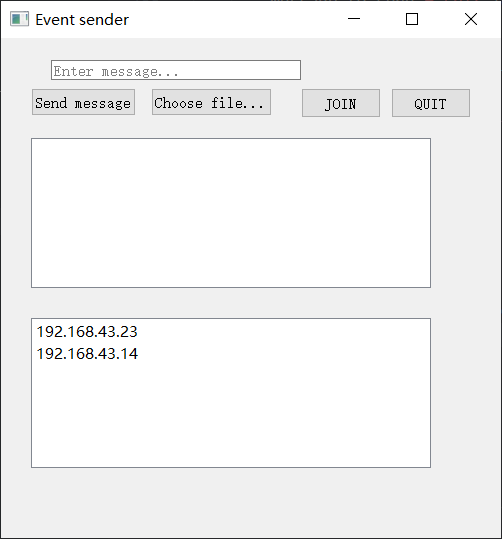
\includegraphics[scale=0.4]{group_mem.png}}
\par{由于在家做实验,所以受到机器数量的限制,本实验的测试只采用两台设备进行。}
\subsection{消息发送测试:}{
\begin{figure}
	\centering
	\begin{minipage}{7cm}
		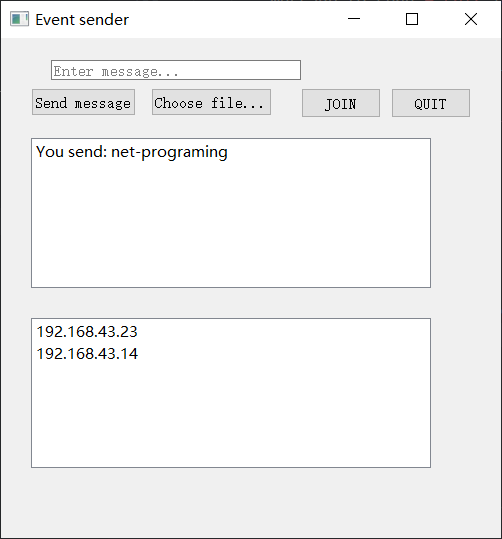
\includegraphics[width=7cm]{send_msg_1.png}
	\end{minipage}
	\begin{minipage}{7cm}
		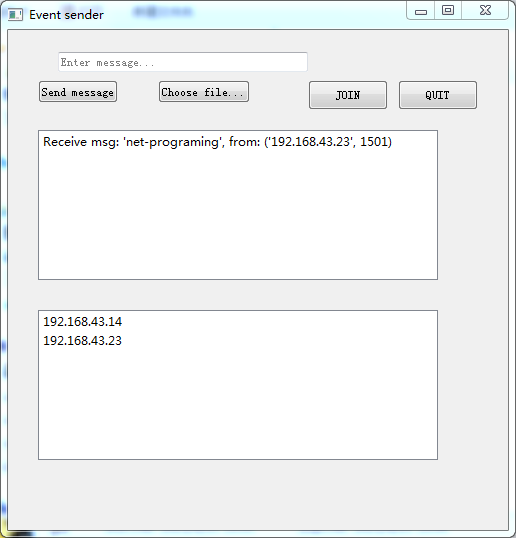
\includegraphics[width=7cm]{rece_msg_1.png}
	\end{minipage}\\
	% 回车
	\begin{minipage}{7cm}
		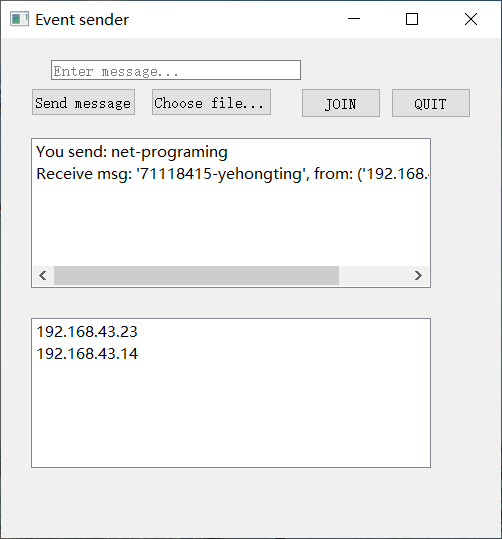
\includegraphics[width=7cm]{rece_msg_2.png}
	\end{minipage}
	\begin{minipage}{7cm}
		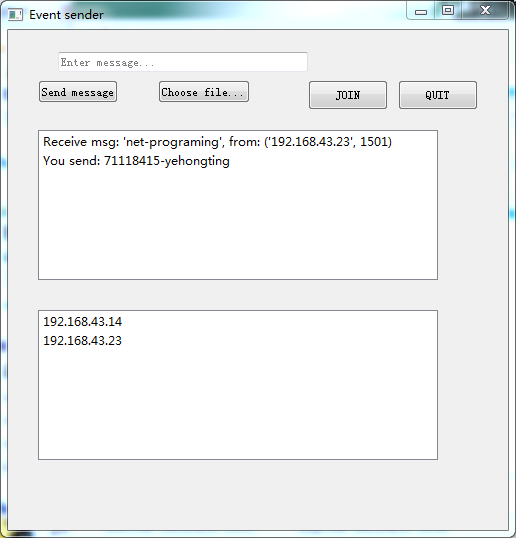
\includegraphics[width=7cm]{send_msg_2.png}
	\end{minipage}
\end{figure}
\par{从下方的四张图片中可以看出,每一方发出的消息都成功的通过多播传输到了组成员处,并且正常显示在界面中。}
}
\\\\\\\\
\subsection{文件发送测试: }{如上图所示,两台机器都能够正常的推送文件,并通过多播发送给每一个成员,并且在接收端可以正确打开。(具体可以自行测试)}
\begin{figure}
	\centering
	\begin{minipage}{7cm}
		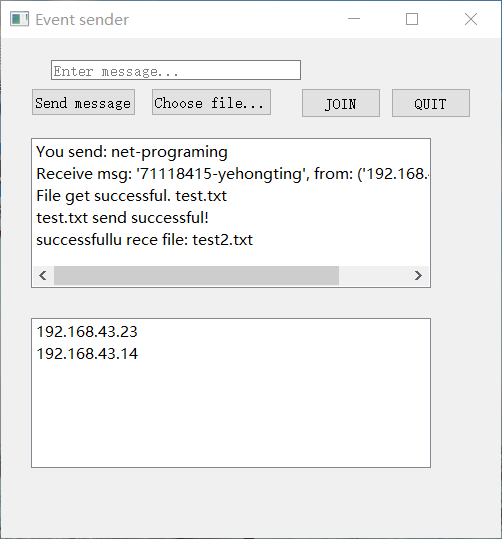
\includegraphics[width=7cm]{A.png}
	\end{minipage}
	\begin{minipage}{7cm}
		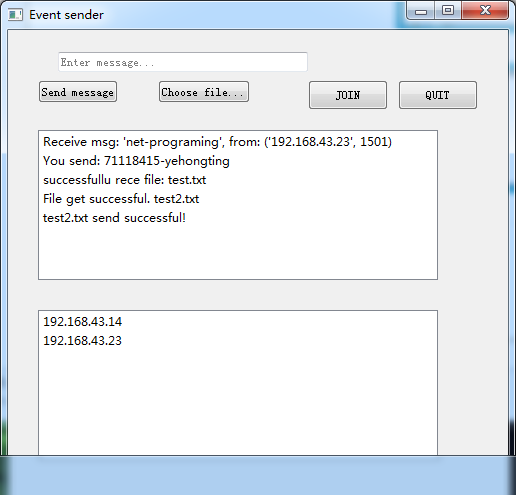
\includegraphics[width=7cm]{B.png}
	\end{minipage}\\
\end{figure}

\subsection{退出多播组测试: }
\par\centerline{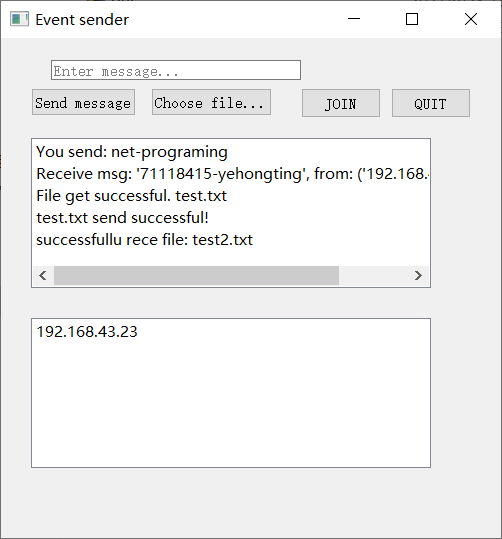
\includegraphics[scale=0.5]{QUIT.png}}
\par{如上图所示,在客户端二退出后,客户端一将会更新成员列表,remove掉退出的客户端。}
\subsection{其余测试: }{其余的测试,可由老师验收时自行测试,请按照README.MD文档中的要求,正确运行程序,否则会导致通信失败等问题。}

\section{总结}
\par{本次大作业,要求完成一个多播聊天工具,通过前期多播作业的基础,因此本次作业完成的较为顺利,在通过一些资料的查询,解决了多个疑难问题。本次作业由于设备等限制,没能在报告中做出良好的展示,稍显不足,不过,本程序的初级版本通过了多机测试,所以最终程序应该也可以完成多播的功能,可以在后期在设备限制解决后进行测试。总体来说,本次作业还是收获颇丰。}
\end{document}
